\tikzstyle{s} = [rectangle, rounded corners, minimum width=2cm, text width=3cm, minimum height=1cm, text centered, draw=black]
\tikzstyle{arrow} = [thick,->,>=stealth]
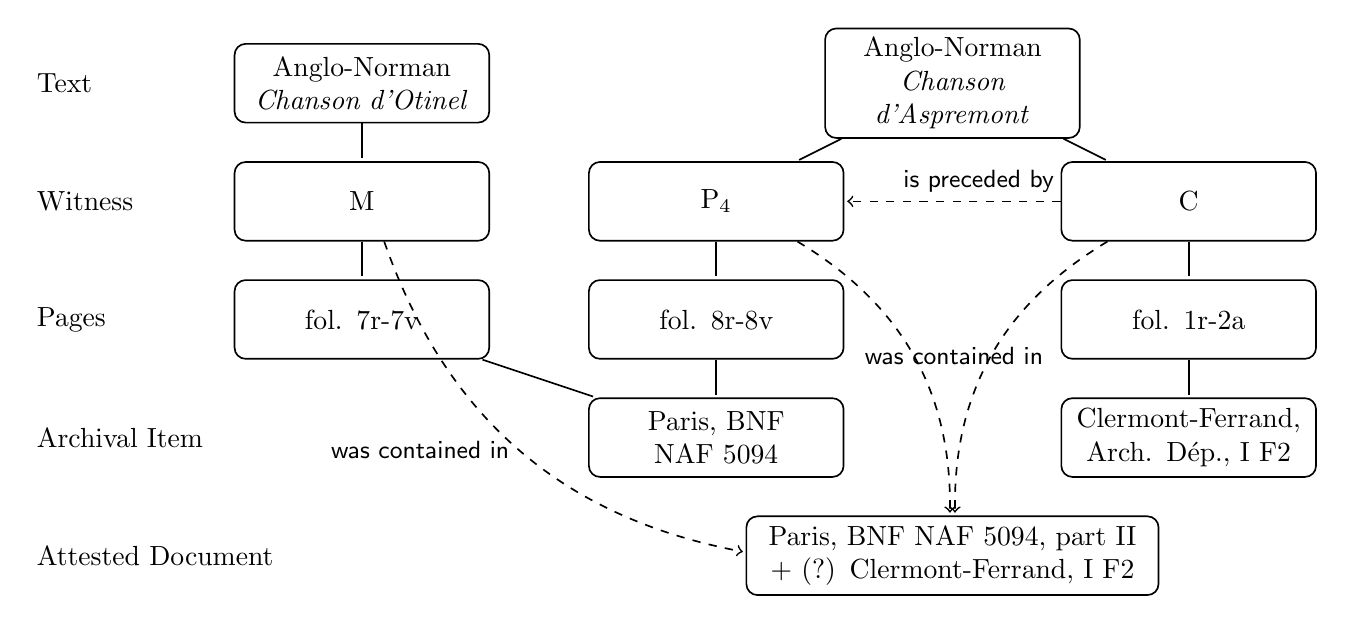
\begin{tikzpicture}[-,shorten >=1pt,auto,node distance=1.5cm,semithick]
\tikzstyle{every state}=[fill=red,draw=none,text=white]

\node[s] (Text) [] {Anglo-Norman \textit{Chanson d'Aspremont}};

\node[s] (P) [below of=Text, xshift=-3cm] {P\textsubscript{4}};
\node[s] (C) [below of=Text, xshift=3cm] {C};
\node[s] (M) [left of=P, xshift=-3cm] {M};
\node[s] (TextOtinel) [above of=M] {Anglo-Norman \textit{Chanson d'Otinel}};
\node [left=1cm, text width=3cm] at (TextOtinel) {Text};
\node [left=1cm, text width=3cm] at (M) {Witness};

\node[s] (PagesP) [below of=P] {fol. 8r-8v};
\node[s] (PagesC) [below of=C] {fol. 1r-2a};
\node[s] (PagesM) [below of=M] {fol. 7r-7v};
\node [left=1cm, text width=3cm] at (PagesM) {Pages};

\node[s] (BNF) [below of=PagesP] {Paris, BNF NAF 5094};
\node[s] (CF) [below of=PagesC] {Clermont-Ferrand, Arch. Dép., I F2};
\node [left=5.5cm, text width=3cm] at (BNF) {Archival Item};

\node[s] (AttestedDoc) [below of=BNF, xshift=3cm, text width=5cm] 
{Paris, BNF NAF 5094, part II + (?) Clermont-Ferrand, I F2};
\node [left=7.5cm, text width=4cm] at (AttestedDoc) {Attested Document};

\path[every node/.style={font=\sffamily\small}]
  (Text) edge node [right] {} (P)
  (Text) edge node [right] {} (C)
  (P) edge node [right] {} (PagesP)
  (C) edge node [right] {} (PagesC)
  (PagesP) edge node [right] {} (BNF)
  (PagesC) edge node [right] {} (CF)
  (P) edge[dashed, ->, bend left=30] node [right, xshift=-0.75cm] {was contained in} (AttestedDoc)
  (C) edge[dashed, ->, bend right=30] node [right] {} (AttestedDoc)
  (C) edge[dashed, ->] node [right, xshift=-0.75cm, yshift=0.25cm] {is preceded by} (P)
  (TextOtinel) edge node [right] {} (M)
  (M) edge node [right] {} (PagesM)
  (PagesM) edge node [right] {} (BNF)
  (M) edge[dashed, ->, bend right=30] node [left] {was contained in} (AttestedDoc)
  ;

\end{tikzpicture}